\documentclass[12pt]{article}
\usepackage{hyperref}
\usepackage{listings}
\usepackage[margin=1in]{geometry}
\usepackage{enumitem}
\usepackage{multicol}
\usepackage{array}
\usepackage{titlesec}
\usepackage{helvet}
\renewcommand{\familydefault}{\sfdefault}
\usepackage{amsmath}     % For math equations
\usepackage{amssymb}     % For advanced math symbols
\usepackage{amsfonts} % For math fonts
\usepackage{gvv}
\usepackage{esint}
\usepackage[utf8]{inputenc}
\usepackage{graphicx}
\usepackage{pgfplots}
\pgfplotsset{compat=1.18}
\titleformat{\section}{\bfseries\large}{\thesection.}{1em}{}
\setlength{\parindent}{0pt}
\setlength{\parskip}{6pt}
\usepackage{multirow}
\usepackage{float}
\usepackage{caption}


\begin{document}

\section*{Problem 12.6}
Compute the 4-point Discrete Fourier Transform (DFT) of the sequence
\begin{align}
x[n] = \{1,0,2,3\}, \quad n=0,1,2,3.
\end{align}


\section*{Input Variables}

\begin{table}[H]
\centering
\begin{tabular}{|c|c|c|}
\hline
\textbf{Symbol} & \textbf{Description} & \textbf{Value} \\
\hline
$N$ & Length of sequence & $4$ \\
\hline
$x[n]$ & Input sequence & $\{1,0,2,3\}$ \\
\hline
$W_N$ & Twiddle factor & $e^{-j2\pi/N}$ \\
\hline
\end{tabular}
\caption{} \label{}
\end{table}

\section*{Solution}

The $N$-point DFT is defined as
\begin{align}
    X[k] &= \sum_{n=0}^{N-1} x[n] \, W_N^{kn}, \quad k=0,1,\dots,N-1,
\end{align}
where
\begin{align}
    W_N = e^{-j \tfrac{2\pi}{N}}.
\end{align}

For $N=4$,
\begin{align}
    W_4 = e^{-j \tfrac{2\pi}{4}} = -j,
\end{align}
so that
\begin{align}
    W_4^0 = 1, \quad W_4^1 = -j, \quad W_4^2 = -1, \quad W_4^3 = j.
\end{align}

The DFT matrix is
\begin{align}
F_4 = \myvec{
1 & 1 & 1 & 1 \\
1 & -j & -1 & j \\
1 & -1 & 1 & -1 \\
1 & j & -1 & -j
}.
\end{align}

The input vector is
\begin{align}
\vec{x} = \myvec{1 \\ 0 \\ 2 \\ 3}.
\end{align}

Thus,
\begin{align}
\vec{X} &= F_4 \, \vec{x}.
\end{align}

Row-by-row computation:
\begin{align}
X[0] &= 1+0+2+3 = 6, \\
X[1] &= 1 + 0(-j) - 2 + 3j = -1+3j, \\
X[2] &= 1 + 0(-1) + 2 - 3 = 0, \\
X[3] &= 1 + 0(j) - 2 - 3j = -1-3j.
\end{align}

Therefore, the DFT vector is
\begin{align}
\vec{X} = \myvec{6 \\ -1+3j \\ 0 \\ -1-3j}.
\end{align}

\section*{Final Answer}
\begin{align}
\vec{X} = \myvec{6 \\ -1+3j \\ 0 \\ -1-3j}
\end{align}

\begin{figure}[H]
    \centering
    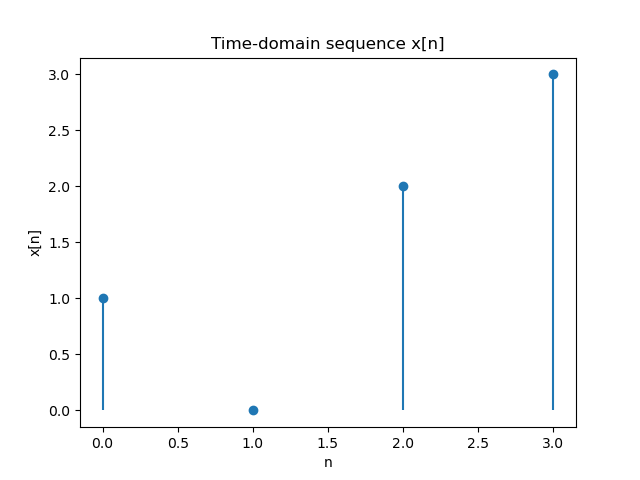
\includegraphics[width=0.7\columnwidth]{figs/fig3.png}
    \caption{}
    \label{fig:placeholder}
\end{figure}

\begin{figure}[H]
    \centering
    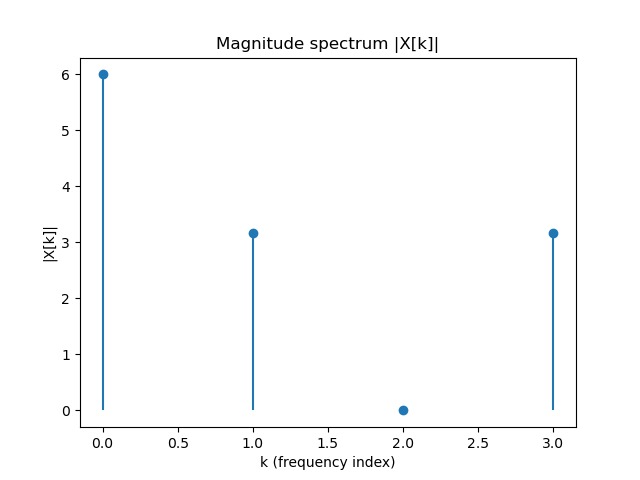
\includegraphics[width=0.7\columnwidth]{figs/fig4.png}
    \caption{}
    \label{fig:placeholder}
\end{figure}

\begin{figure}[H]
    \centering
    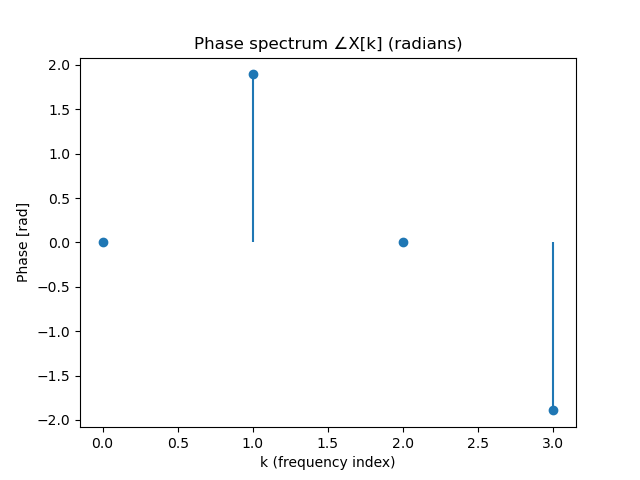
\includegraphics[width=0.7\columnwidth]{figs/fig5.png}
    \caption{}
    \label{fig:placeholder}
\end{figure}


\end{document}
